% Copyright © 2015-2016 Martin Ueding <dev@martin-ueding.de>
%
\documentclass[english, fleqn]{beamer}


\usetheme{Malmoe}
\useoutertheme{infolines}
\usepackage[bibatend]{header}

\newcommand\qqandqq{\qquad\text{and}\qquad}

\DeclareSIUnit\year{yr}

\AtBeginSection[]
{
    \begin{frame}
        \sectionpage
        \tableofcontents[sectionstyle=show/shaded, subsectionstyle=show/shaded/hide, subsubsectionstyle=hide/hide/hide]
    \end{frame}
}

\AtBeginSubsection[]
{
    \begin{frame}
        \subsectionpage
        \tableofcontents[sectionstyle=show/shaded, subsectionstyle=show/shaded/hide, subsubsectionstyle=hide/hide/hide]
    \end{frame}
}

\renewcommand\iup{\text i}
\renewcommand\eup{\text e}


\setbeamertemplate{navigation symbols}{}
\addtobeamertemplate{navigation symbols}{}{%
    \usebeamerfont{footline}%
    \usebeamercolor[fg]{footline}%
    \hspace{1em}%
    \insertframenumber/\inserttotalframenumber
}

\graphicspath{{_build/}{Figures/}}

\title{Nucleon Decay}
%\subtitle{}
\author{Martin Ueding -- mu@martin-ueding.de}
%\date{}

\begin{document}

\begin{frame}
    \titlepage
\end{frame}

\begin{frame}
    \frametitle{Standard model}

    \begin{columns}[t]
        \begin{column}{.3\linewidth}
            \begin{block}{Fermions}
                \

                \begin{tabular}{ccc}
                    u & c & t \\
                    d & s & b \\
                    \midrule
                    $\nuup_\mathsf e$ & $\nuup_\muup$ & $\nuup_\tauup$ \\
                    $\mathsf e^-$ & $ \muup^-$ & $\tauup^-$
                \end{tabular}
            \end{block}
        \end{column}
        \begin{column}{.7\linewidth}
            \begin{block}{Bosons}
                \

                \begin{tabular}{llll}
                    Group & Force & Property & Carrier \\
                    \midrule
                    $\mathsf{SU}(3)$ & Strong & Color & Gluon \\
                    $\mathsf{SU}(2)$ & Weak & Weak Isospin & W, Z \\
                    $\mathsf{SU}(1)$ & EM & Hypercharge & B, $\gammaup$
                \end{tabular}
            \end{block}
        \end{column}
    \end{columns}

    \

    \begin{block}{Gauge group}
        $\mathsf{SU}(3) \times \mathsf{SU}(2) \times \mathsf{SU}(1)$
    \end{block}

\end{frame}

\section{Grand unified theories}

\subsection{Motivation}

\begin{frame}
    \frametitle{Charges}

    Quarks and leptons electric charges are very related:
    \[
        \frac{Q(\mathsf u)}{Q(\mathsf e^+)} = \frac 23
        \qqandqq
        \frac{Q(\mathsf d)}{Q(\mathsf e^+)} = - \frac 13
    \]

    \pause

    And most strikingly:
    \[
        \frac{Q(\mathsf p)}{Q(\mathsf e^+)} = 1
    \]

    \pause

    \begin{itemize}
        \item QED does not need this
        \item Begs for unification
        \item Be careful with anthropic principle!
    \end{itemize}
\end{frame}

\begin{frame}
    \frametitle{Number of particles}

    \begin{itemize}
        \item Two quarks per generation
        \item Two leptons per generation
        \item Three generations of quarks and leptons
    \end{itemize}
\end{frame}

\begin{frame}
    % TODO Does this really apply?

    \frametitle{Matter and anti-matter asymmetry}

    Why is there more matter than anti-matter?

    Standard model is symmetric

    Violation via GUT process?
\end{frame}

\subsection{Georgi-Glashow model}

\begin{frame}
    Particles are basis vectors of irreps.
\end{frame}

\begin{frame}
    \frametitle{Multiplets of SU(5)}
    \[
        \begin{pmatrix}
            \bar\nuup_\mathsf L
        \end{pmatrix}
        \qquad
        \begin{pmatrix}
            \mathsf e^+_\mathsf R \\
            \bar\nuup_\mathsf R \\
            \mathsf d_\mathsf R
        \end{pmatrix}
        \qquad
        \begin{pmatrix}
            \mathsf e^+_\mathsf L \\
            \mathsf u_\mathsf L \\
            \mathsf d_\mathsf L \\
            \bar{\mathsf u}_\mathsf L
        \end{pmatrix}
        \qquad
        \begin{pmatrix}
            \mathsf e^-_\mathsf R \\
            \bar{\mathsf u}_\mathsf R \\
            \bar{\mathsf d}_\mathsf R \\
            \mathsf u_\mathsf R
        \end{pmatrix}
        \qquad
        \begin{pmatrix}
            \nuup_\mathsf L \\
            \mathsf e^-_\mathsf L \\
            \bar{\mathsf d}_\mathsf L
        \end{pmatrix}
        \qquad
        \begin{pmatrix}
            \nuup_\mathsf R
        \end{pmatrix}
    \]
\end{frame}

\subsection{Pati-Salam model}

\begin{frame}
    %\parencite{Wu/Proton_decay}
\end{frame}

\section{Proton decay}

\begin{frame}
    \frametitle{Standard model}

    \begin{columns}[t]
        \begin{column}{.5\linewidth}
            \begin{block}{Neutron decay}
                We have $\mathsf n \to \mathsf p + \mathsf e^- \bar\nuup_{\mathsf e}$:

                \

                \includegraphics{beta}
            \end{block}
        \end{column}
        \pause
        \begin{column}{.5\linewidth}
            \begin{block}{Proton decay}
                \begin{itemize}
                    \item Proton is lightest nucleon
                    \item \alert{Proton is stable in standard model}
                \end{itemize}
            \end{block}
        \end{column}
    \end{columns}
\end{frame}

\subsection{Pion + positron}

\begin{frame}
    \frametitle{The X boson}

    \begin{columns}[t]
        \begin{column}{.5\textwidth}
            \begin{block}{Decay modes}
                \begin{gather*}
                    \mathsf X \to \mathsf u + \mathsf u \\
                    \mathsf X \to \mathsf e^+ + \bar{\mathsf d}
                \end{gather*}
            \end{block}
        \end{column}
        \begin{column}{.5\textwidth}
            \begin{block}{Properties}

                \

                \begin{tabular}{ll}
                    Mass & $\approx \SI{e15}{\giga\electronvolt}$ \\
                    Electric charge & $+4/3$ \\
                    Color charge & triplet \\
                    Spin & 1 \\
                    Weak isospin $z$ & $+1/2$ \\
                    Hypercharge & $5/3$ \\
                    $B - L$ & $2/3$
                \end{tabular}
            \end{block}
        \end{column}
    \end{columns}

    % TODO https://en.wikipedia.org/wiki/X_and_Y_bosons
\end{frame}

\begin{frame}
    \frametitle{Proton decay via X boson}

    \begin{center}
        \includegraphics{proton-x-pi-1}
        \hfill
        \includegraphics{proton-x-pi-2}
    \end{center}

    Gives $\mathsf p \to \piup^0 + \mathsf e^+$
\end{frame}


\section{Experiments}

\subsection{Quick estimation}

\begin{frame}
    \begin{block}{Observation}
        Our bodies are not very radioactive.
    \end{block}

    \pause

    \begin{block}{Proton lifetime}
        \begin{itemize}
            \item We would notice \SI{1}{\gray\per\year}
            \item Body consists half of protons
            \item Proton lifetime greater than \SI{7e23}{\second} or \SI{2e16}{\year}
        \end{itemize}
    \end{block}

    \nocite{wikipedia/groessenordnung-aequivalentdosis}
\end{frame}

\subsection{Super Kamiokande}

\begin{frame}
    \frametitle{Setup}

    \begin{itemize}
        \item Cylinder, \SI{39.3}{\meter} diameter, \SI{41.4}{\meter} height
        \item \SI{50}{\kilo\tonne} ultra pure water
        \item \num{13000} photo multipliers
        \item \SI{1000}{\meter} under ground
        \item Located in Kamioka-mine, Hida-city, Gifu, Japan
    \end{itemize}

    % TODO http://www-sk.icrr.u-tokyo.ac.jp/sk/sk/index-e.html
\end{frame}

\begin{frame}
    \frametitle{}

\end{frame}

\begin{frame}
    \frametitle{Example proton decay event}

    \centering
    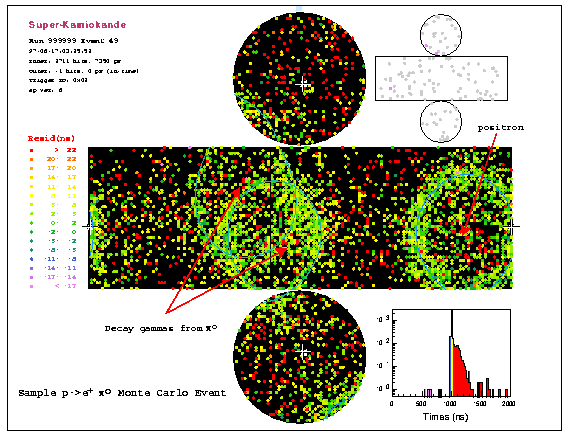
\includegraphics[width=0.8\linewidth]{Figures/epi0_nice_event.png}
    % TODO http://hep.bu.edu/~superk/pdk.html
\end{frame}

\begin{frame}
    \titlepage
\end{frame}


\section*{References}

\begin{frame}

    \nocite{tikz-feynman}

    \printbibliography
\end{frame}

\end{document}

% vim: spell spelllang=en_us
